\textbf{Teste 1}\\
Identificação de jogadores utilizando os pontos de interesses.

\begin{figure}
    \centering
    \caption{\label{fig_comparativo_img}A imagem (A) é a original, e as representações em vermelho são seus pontos de interesse. A imagem (B) é o resultado da detecção por bordas e seus pontos similares com a imagem (A).}
    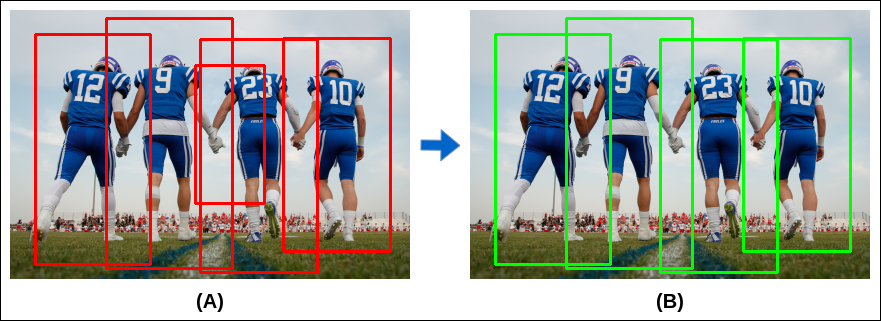
\includegraphics[scale=0.3]{05-SLIDES_DESENVOLVIMENTO/Etapa_de_Testes/imagens_testes/comparativo_imagem.png}
\end{figure}